\begin{frame}{Optimierung der Übertragungsfunktion}

\uncover<2->{
Idee: Iterative Anpassung mit
\begin{align*}
			\underline{H}^{i+1} \left( \omega \right) = \underline{H}^{i} \left( \omega \right) \left( 1+ \sigma_H \cdot \left( \frac{\underline{U}_{out,\mathrm{mess}}^{i} \left( \omega \right) }{\underline{U}_{out,\mathrm{ideal}}^{i} \left( \omega \right) } -1 \right) \right) 
		\end{align*}
mit $ \sigma_H $ als Schrittweite.
}
\begin{itemize}
\uncover<3->{
\item Fokus auf Optimierung des Betrags nach ersten Messungen mit Phasenanpassung
}
\end{itemize}

\uncover<4>{
	\begin{picture}(0, -40)
	\put(120, -30){
		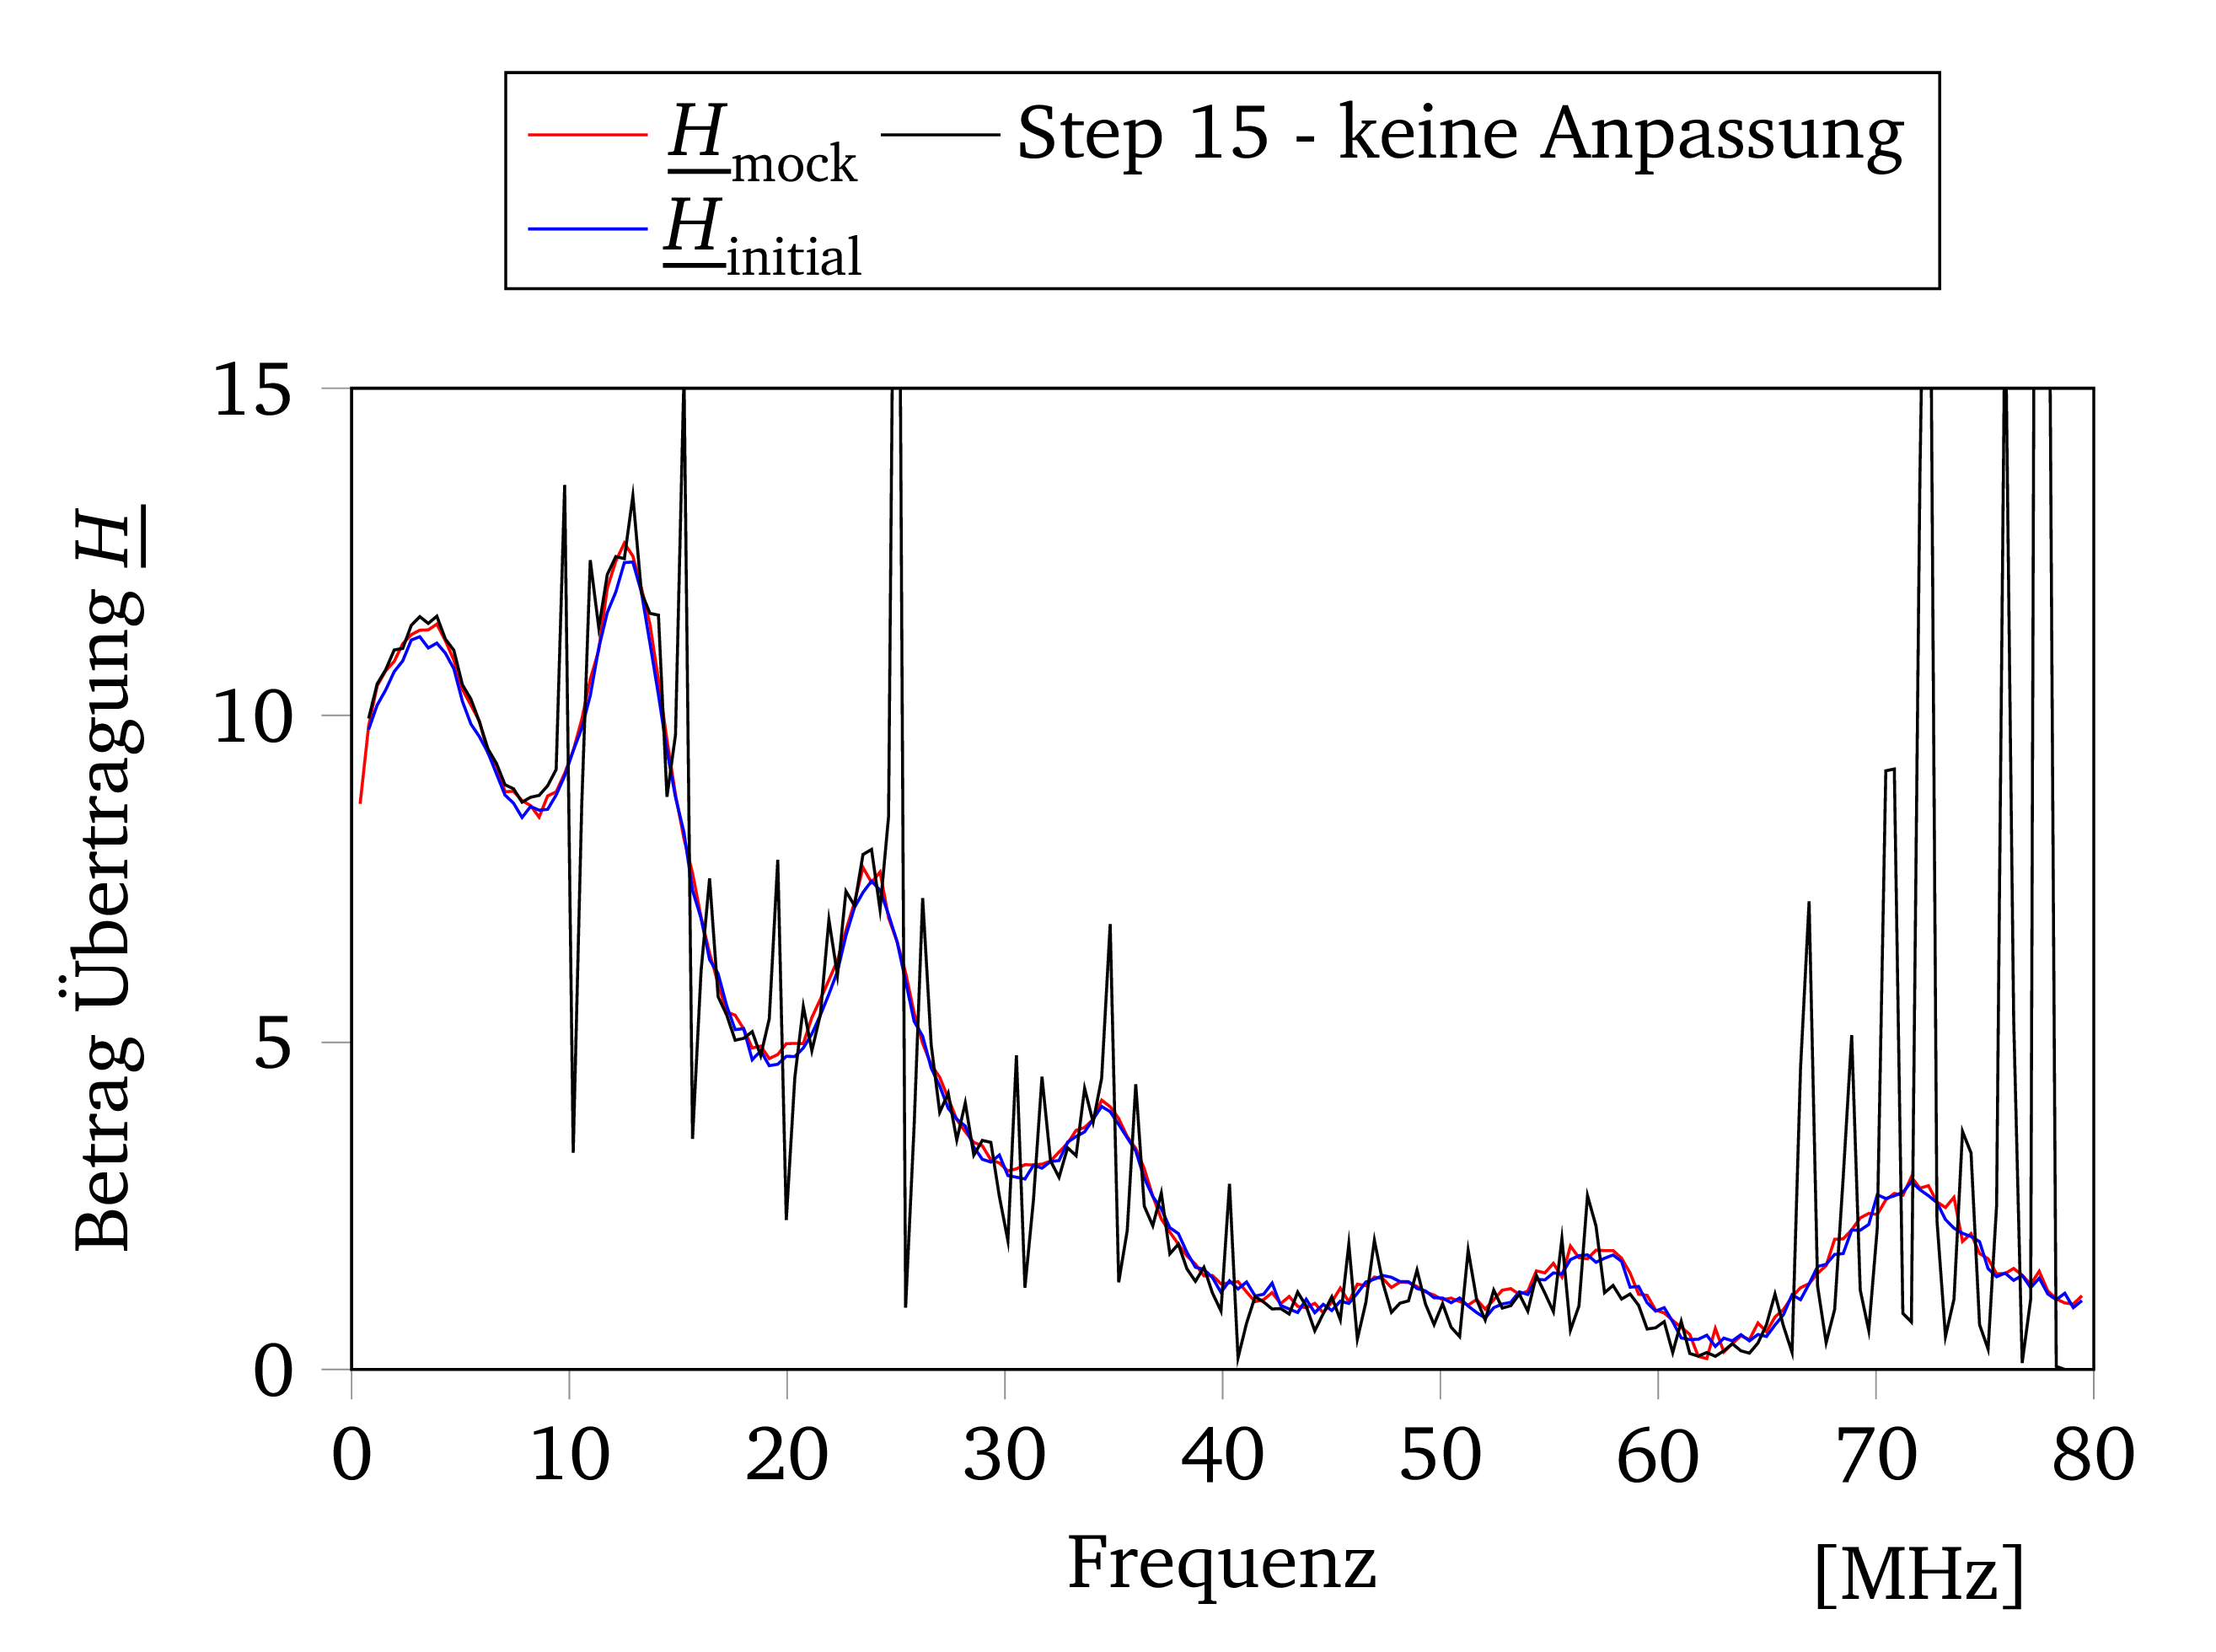
\includegraphics[scale=0.7]{slides/adjust_H/adjust_H_mock.png}	
	}
\end{picture}	
}

%\uncover<2-4, 5->{
%	\begin{picture}(0,70)
%		\put(15,5){
%			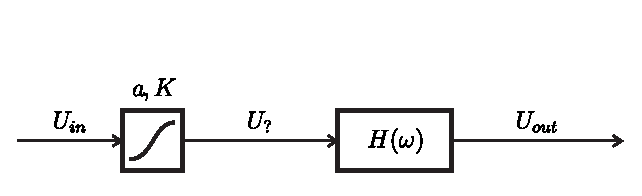
\includegraphics[scale=1.0]{slides/Problemstellung/Slide1.eps} 
%		}
%	\end{picture}
%	}
%

\end{frame}



